\section{Activités}

Le développement du projet peut se découper en plusieurs phases, qui elles-mêmes se divisent en plusieurs activités. Voici la liste de ces activités :

\begin{enumerate}
	\item Analyse
	\begin{enumerate}
		\item Item 1
		\item Item 2
	\end{enumerate}
	\item Conception
	\begin{enumerate}
		\item Item 1
		\item Item 2
	\end{enumerate}
	\item Implémentation
	\begin{enumerate}
		\item Item 1
		\item Item 2
	\end{enumerate}
	\item Résultats
	\begin{enumerate}
		\item Item 1
		\item Item 2
	\end{enumerate}
\end{enumerate}

\section{Planification}
Le projet comporte une série de dates-clé qu’il est important de respecter :
\begin{center}
   \begin{tabular}{ | l | c | r | }
     \hline
		Date & Semaine & Tâche \\ \hline
		\color{red}Lundi 18 septembre 2017 & Semaine P1 & Début du projet \\ \hline
		\color{red}Vendredi 9 février 2018 & Semaine P15 & Dépôt du rapport \\ \hline
		\color{red}26 février-9 mars 2017 & - & Défense orale \\ \hline
     \hline
   \end{tabular}
\end{center}

Les dates en rouge sont des dates de rendu officielles.
Les autres représentent des jalons dans l’avancement du projet.

\section{Diagramme de Gantt}
	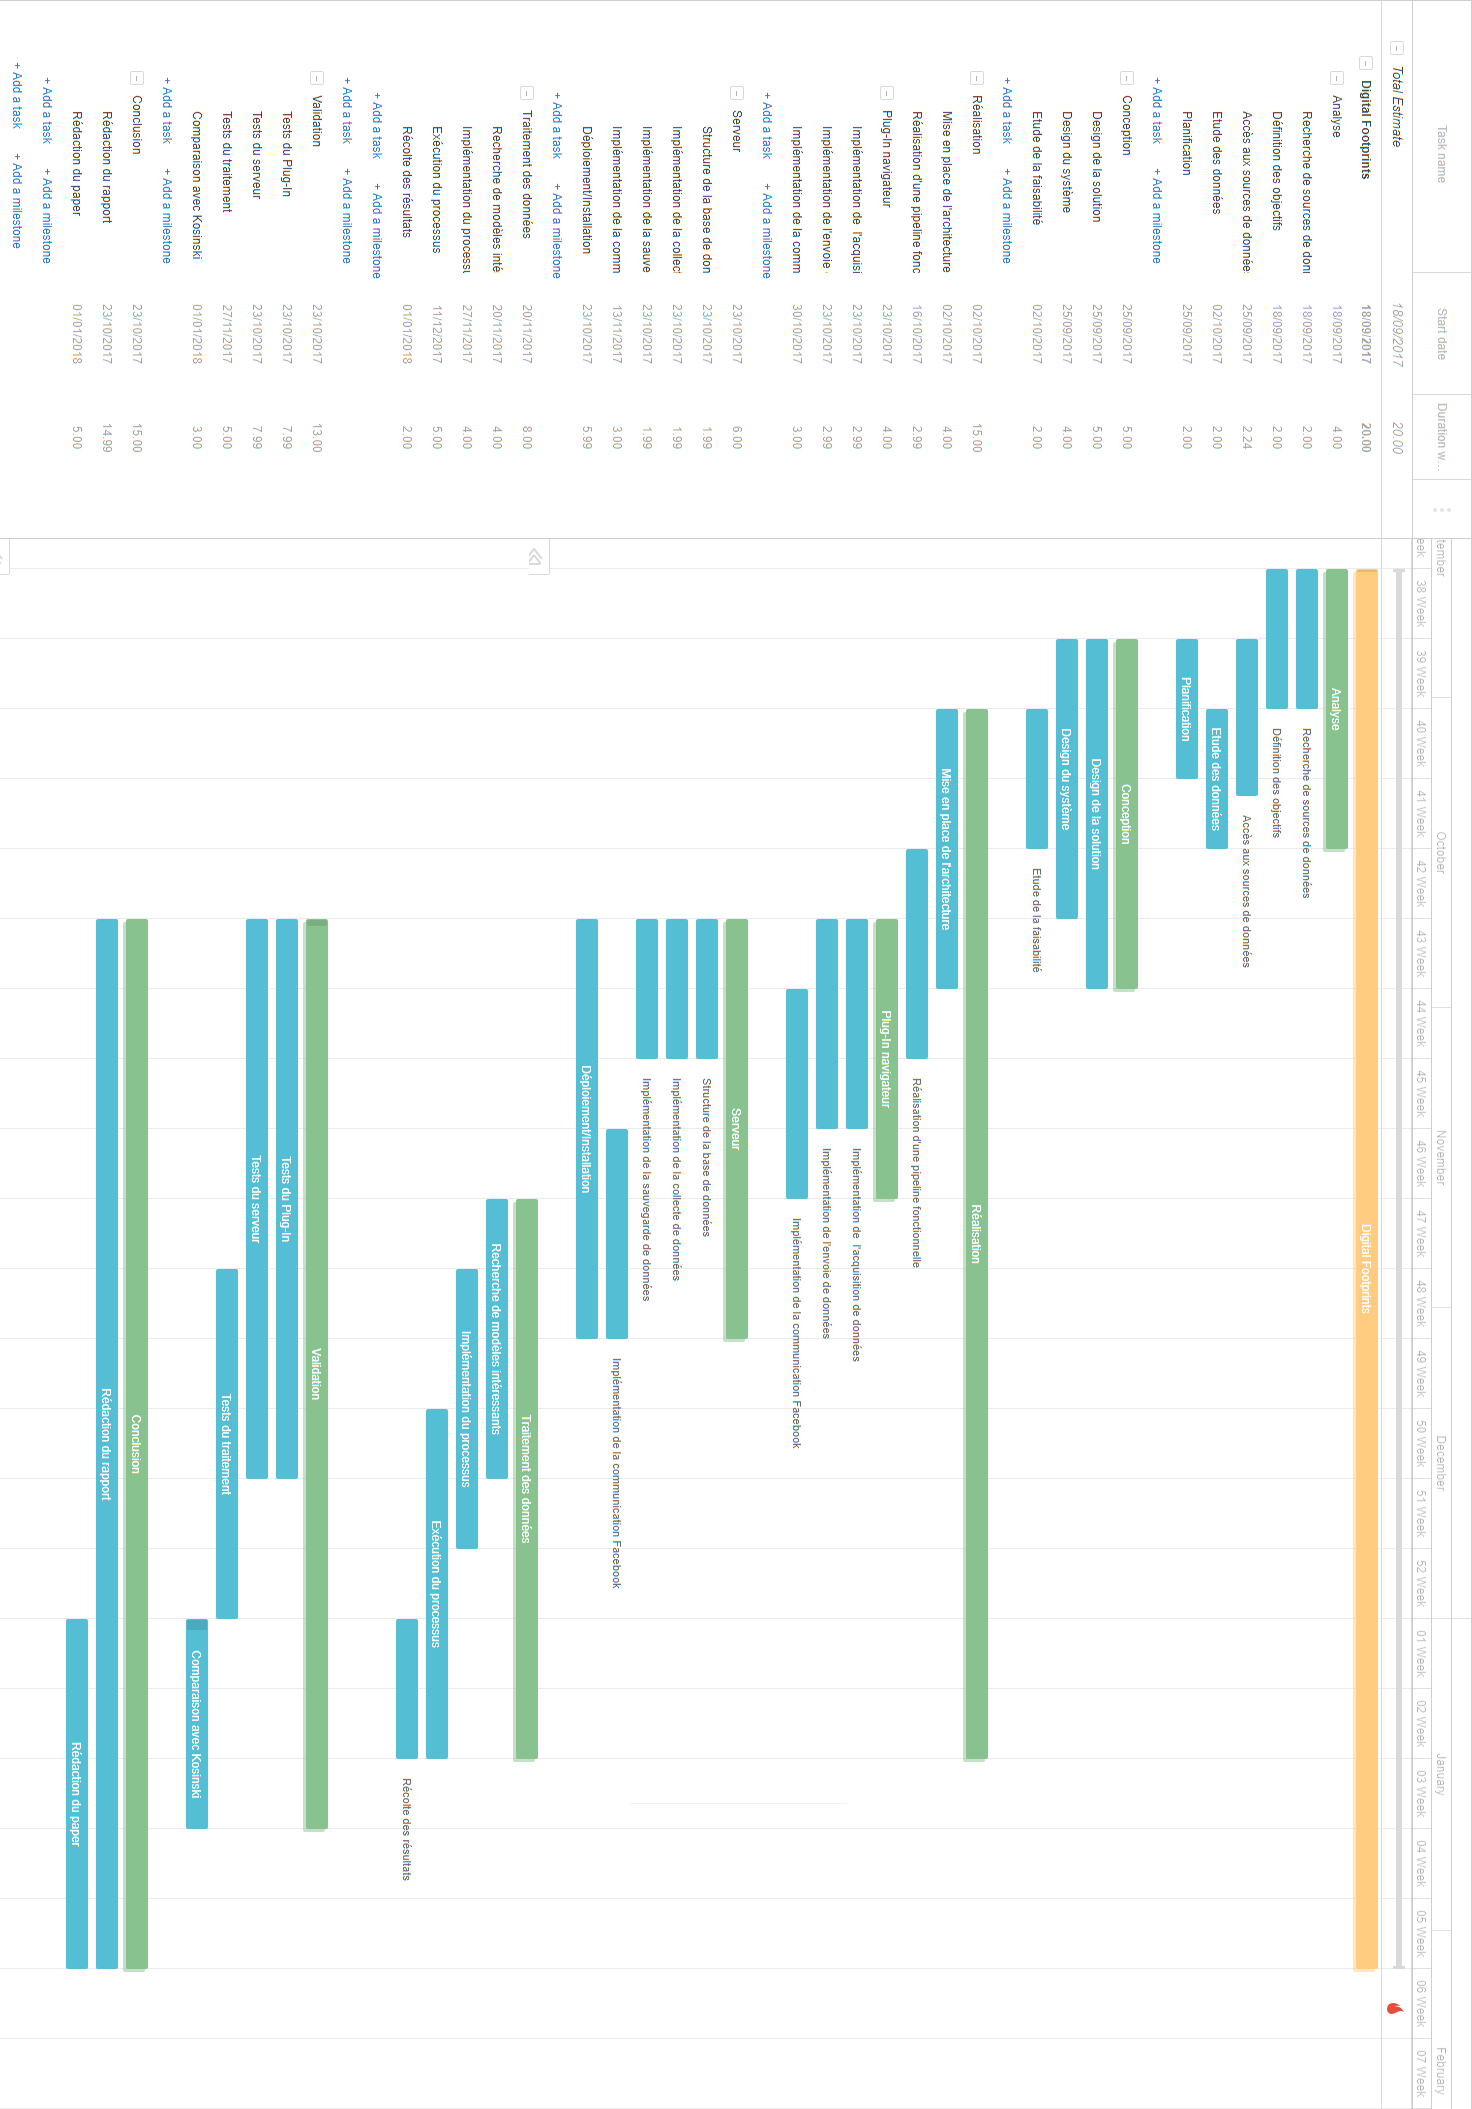
\includegraphics[width=0.85\textwidth]{images/annexes/cdc/gantt}